\chapter{$L^{p}$~空间$^*$}

前面章节告诉我们: 连续(或几乎处处连续)函数及其相应的黎曼积分理论的地位和作用, 在一定意义上已被可测函数及其勒贝格积分理论所代替. 新的积分理论不仅扩大了积分的对象, 而且新的~L-可积函数类的全体还呈现出与欧氏空间极其类似的结构与性质, 从而为我们在其上建立分析学奠定了基础.

所有~$p$~次幂~L-可积函数的全体构成的空间, 称为~$L^p$~空间. $L^p$~空间是里斯于~1910~年引入的, 他所使用的主要工具是赫德尔不等式以及闵可夫斯基不等式
\footnote{这些不等式最初是数列形式给出的, 由里斯将其推广到积分形式.}. 在勒贝格积分理论创立后, $L^2$~空间的重要性立即被人们所认识, 这是因为它紧密联系着傅里叶级数及其它的展开式. $L^p$~空间理论主要研究~L-可积函数类的整体结构及其相互关系.

我们知道在实数空间~$\R$~中, 有理数处处稠密, 且全体有理数是可列的, 此性质称为实数空间的可分性．同时, 实数空间还具有完备性, 即其中任何柯西列必收敛于某实数. 在空间理论的研究中, 可分性(可通过研究稠密子空间来研究整个空间)和完备性
(保证柯西列收敛的极限点跑不出该空间范围)是两个重要的性质, 本章将讨论~$L^p$~空间的完备性与可分性.

$L^p$~空间理论的应用涉及微分方程、积分方程、傅里叶分析、有限元分析等许多领域. 另外, 与~$L^p$~空间对应的~$\ell^p$空间是由~$p$~次幂可和的序列组成的空间, 在泛函分析和拓扑向量空间中, 他们构成了巴拿赫空间一类重要的例子.

本章所论述的内容既可以看成是勒贝格积分理论的应用, 也为学习后续课程
《泛函分析》提供了方便和模型.

\section{$L^2$~空间基本概念及不等式}

\subsection*{一、基本概念及不等式}

\begin{Definition}\label{Def-6-2}

设~$f(x)$~为~$\left[a,\,b\right]$~上的可测函数, 满足
\[
\int_{a}^{b}f^{2}(x)\mathrm{d}\mu<+\infty
\]
则称~$f(x)$~为平方~L-可积函数. 所有平方~L-可积函数的全体记为~$L^2[a,\,b]$\index{$L^2$~空间}.
\end{Definition}

\begin{Proposition}\label{Pro-6-1}

$L^2[a,\,b]\subset L[a,\,b]$.
\end{Proposition}

\begin{proof}
由不等式
\[
|f(x)|\leqslant \frac{1+f^{2}(x)}{2}
\]
可知该命题成立.
\end{proof}

\begin{Theorem} \label{thm-6-1}
(\textbf{施瓦兹不等式}\index{施瓦兹不等式}) 设~$f(x), g(x)\in L^2[a,\,b]$, 则
\[
\int_{a}^{b}f(x)g(x)\mathrm{d}\mu \leqslant \Big[\int_{a}^{b}f^{2}(x)\mathrm{d}\mu\Big]^{\frac{1}{2}}\Big[\int_{a}^{b}g^{2}(x)\mathrm{d}\mu\Big]^{\frac{1}{2}}
\]
\end{Theorem}

\begin{proof}
不妨设~$\int_{a}^{b}f^{2}(x)\mathrm{d}\mu>0$. 事实上, 若~$\int_{a}^{b}f^{2}(x)\mathrm{d}\mu=0$, 则函数~$f(x)$~在区间~$\left[a,\,b\right]$~上几乎处处为~0, 则上述不等式两端都为~0, 显然成立.
令
\begin{eqnarray*}
F(z)&=&\int_{a}^{b}\big[z f(x)+g(x)\big]^{2}\mathrm{d}\mu \\
&=& z^{2}\int_{a}^{b}f^{2}(x)\mathrm{d}\mu+2z\int_{a}^{b}f(x)g(x)\mathrm{d}\mu+\int_{a}^{b}g^{2}(x)\mathrm{d}\mu
\end{eqnarray*}
易知对所有~$z$, $F(z)\geqslant 0$. 注意到二次实系数多项式
\[
F(z)=Az^{2}+2Bz+C,\quad A>0
\]
若对所有~$z$, 有~$F(z)\geqslant 0$, 则一定有~$B^{2}\leqslant AC$. 否则将产生矛盾
\[
F\Big(-\frac{B}{A}\Big)=\frac{1}{A}(AC-B^{2})<0
\]
因此, 可得
\[
\Big[\int_{a}^{b}f(x)g(x)\mathrm{d}\mu\Big]^{2} \leqslant \Big[\int_{a}^{b}f^{2}(x)\mathrm{d}\mu\Big]\Big[\int_{a}^{b}g^{2}(x)\mathrm{d}\mu\Big]
\]
定理证毕.
\end{proof}



\begin{Corollary}\label{cor-6-1}
设~$f(x) \in L^2[a,\,b]$, 则
\[
\int_{a}^{b}|f(x)|\mathrm{d}\mu \leqslant \sqrt{b-a}\sqrt{\textstyle{\int_{a}^{b}f^{2}(x)\mathrm{d}\mu}}
\]
\end{Corollary}

\begin{proof}
只需在定理~\ref{thm-6-1}~中令~$f(x)=|f(x)|$, $g(x)=1$~即得.
\end{proof}

\begin{Theorem} \label{thm-6-2}
(\textbf{柯西不等式}\index{柯西不等式}) 设~$f(x), g(x)\in L^2[a,\,b]$, 则
\[
\sqrt{\textstyle{\int_{a}^{b}\big[f(x)+g(x)\big]^{2}\mathrm{d}\mu}} \leqslant \sqrt{\textstyle{\int_{a}^{b}f^{2}(x)\mathrm{d}\mu}}+\sqrt{\textstyle{\int_{a}^{b}g^{2}(x)\mathrm{d}\mu}}
\]
\end{Theorem}


\begin{proof}
由施瓦兹不等式
\[
\int_{a}^{b}f(x)g(x)\mathrm{d}\mu \leqslant \Big[\int_{a}^{b}f^{2}(x)\mathrm{d}\mu\Big]^{\frac{1}{2}}\Big[\int_{a}^{b}g^{2}(x)\mathrm{d}\mu\Big]^{\frac{1}{2}}
\]
则
\begin{eqnarray*}
&& \int_{a}^{b}f^{2}(x)\mathrm{d}\mu+\int_{a}^{b}g^{2}(x)\mathrm{d}\mu+2\int_{a}^{b}f(x)g(x)\mathrm{d}\mu \\
&\leqslant& \int_{a}^{b}f^{2}(x)\mathrm{d}\mu+\int_{a}^{b}g^{2}(x)\mathrm{d}\mu+2\Big[\int_{a}^{b}f^{2}(x)\mathrm{d}\mu\Big]^{\frac{1}{2}}
\Big[\int_{a}^{b}g^{2}(x)\mathrm{d}\mu\Big]^{\frac{1}{2}}
\end{eqnarray*}
即得
\[
\int_{a}^{b}\big[f(x)+g(x)\big]^{2}\mathrm{d}\mu\leqslant \Big(\sqrt{\textstyle{\int_{a}^{b}f^{2}(x)\mathrm{d}\mu}}+\sqrt{\textstyle{\int_{a}^{b}g^{2}(x)\mathrm{d}\mu}}\Big)^{2}
\]
定理证毕.
\end{proof}

柯西不等式使我们从一个新的视角来研究~$L^2[a,\,b]$.

\begin{Definition}
设~$X$~为线性空间, 若对任意的~$x \in X$, 都有一个正实数~$\|x\|$~与之对应, 且满足:

(i) $\|x\|\geqslant 0$, 且~$\|x\|= 0$~当且仅当~$x$~为~$X$~中的零元;

(ii) $\|kx\|=|k|\|x\|$, 其中~$k\in \mathbb{R}$;

(iii) $\|x+y\|\leqslant \|x\|+\|y\|$.

\noindent 则称~$\|\cdot\|$~为~$X$~上的一个范数\index{范数}, 定义了范数的线性空间~$(X,\,\|\cdot)$~称为赋范线性空间\index{赋范线性空间}.
\end{Definition}

\setcounter{footnote}{0}

若~$f(x)\in L^2[a,\,b]$, 令
\[
\|f\|=\sqrt{\textstyle{\int_{a}^{b}f^{2}(x)\mathrm{d}\mu}}
\]
$\|f\|=0$~当且仅当~$f$~几乎处处为~0\footnote{在~$L^2[a,\,b]$~中, 几乎处处为零的函数视为与零等价, 可看作零函数.}, 易知~$\|\cdot\|$~满足范数定义中的三条性质故是一个范数, 从而~$\big(L^p[a,b],\|\cdot\|\big)$~构成赋范线性空间. 利用范数~$\|\cdot\|$~可以在~$L^2[a,\,b]$~中自然诱导距离, 即
\[
d(f,\,g)=\|f-g\|
\]
在第一章~$\S1.5$~中, 我们已经介绍了距离的有关性质, 这里不再重复. $L^2[a,\,b]$~按距离~$d$~成为一个距离空间(或度量空间), 这种观点最初是由希尔伯特提出的, 因此, $L^2[a,\,b]$~也称为希尔伯特空间.

\medskip

\subsection*{二、依范数收敛}

\begin{Definition}\label{Def-6-3}
设~$f_{1}, f_{2}, \cdots, f_{n}, \cdots$~和~$f$~都是~$L^{2}\left[a,\,b\right]$~中的函数, 若对任意的~$\varepsilon>0$, 存在自然数~$N$, 当~$n>N$~时, 有
\[
\|f_{n}-f\|<\varepsilon
\]
则称~$\{f_{n}\}$~依范数收敛\index{依范数收敛}于~$f$, 称~$f$~为~$\{f_{n}\}$~的极限. 记为~$\lim\limits_{n\rightarrow \infty}f_{n}=f$~或~$f_{n}\xrightarrow{\mathrm{\|\cdot\|}} f$.
\end{Definition}

\begin{Remark}
$\lim\limits_{n\rightarrow \infty}f_{n}(x)=f(x)$~与~$\lim\limits_{n\rightarrow \infty}f_{n}=f$~所代表的意义是不同的, 前者表示对固定的元素~$x$, 数列~$\{f_{n}(x)\}$
~收敛于~$f(x)$. 而后者表示
\[
\lim\limits_{n\rightarrow \infty}\int_{a}^{b}\big[f_n(x)-f(x) \big]^{2}\mathrm{d}\mu=0
\]
这种收敛方式也称为函数列~$\{f_{n}(x)\}$~均方收敛于~$f(x)$.
\end{Remark}

\begin{Theorem}
设~$f_{1}, f_{2}, \cdots, f_{n}, \cdots$~和~$f$~都是~$L^{2}\left[a,\,b\right]$~中的函数, $f_{n}\xrightarrow{\mathrm{\|\cdot\|}} f$, 则
~$f_n \xrightarrow{~\mu~} f$.
\end{Theorem}

\begin{proof}
对任意的~$\varepsilon>0$, 令
\[
E_n(\varepsilon) = \big\{ x \in E: \: |f_n(x) - f(x)| \geqslant \varepsilon \big\}
\]
则
\[
\int_{a}^{b}\left[f_n(x)-f(x)\right]^{2}\mathrm{d}\mu\geqslant \int_{E_n(\varepsilon)}\left[f_n(x)-f(x) \right]^{2}\mathrm{d}\mu\geqslant \varepsilon^{2}\cdot m\big(E_n(\varepsilon)\big)
\]
因此, 当~$n\rightarrow \infty$~时, 有
\[
m\big(E_n(\varepsilon)\big)\rightarrow 0
\]
故~$f_n \xrightarrow{~\mu~} f$.
\end{proof}

\begin{Theorem}
设~$f_{1}, f_{2}, \cdots, f_{n}, \cdots$~和~$f$~都是~$L^{2}\left[a,\,b\right]$~中的函数, $f_{n}\xrightarrow{\mathrm{\|\cdot\|}} f$, 则
必存在子列~$\{f_{n_k}\} \subset \{f_n\}$~使得~$f_{n_k} \xrightarrow{\mathrm{a.e.}} f$.
\end{Theorem}

\begin{proof}
由里斯定理可得.
\end{proof}

\begin{Remark}
一方面, 由第三章~$\S3.2$~的例~2~可知
\[
f_{n}\xrightarrow{\mathrm{\|\cdot\|}} f \nRightarrow f_{n}\xrightarrow{\mathrm{a.e.}} f
\]
另一方面, $f_{n}$~点点收敛于~$f$~也推不出~$f_{n}$~依范数收敛于~$f$.
\end{Remark}


\begin{Example}
设定义在闭区间~$[0,\,1]$~上的函数列~$f_{n}(x)$~为
\[
f_{n}(x) = \left\{ \!\!
\begin{array}{ll}
n, & 0<x<\dfrac{1}{n}  \\[0.3cm]
0, & x \mbox{~为~} [0,\,1] \mbox{~上的其他点}
\end{array}
\right.
\]
显然
\[
\lim\limits_{n\rightarrow\infty}f_n(x)=0,\quad \forall x\in [0,\,1]
\]
但
\[
\int_{0}^{1}f_{n}^{2}(x)\mathrm{d}\mu=\int_{0}^{\frac{1}{n}}n^{2}\mathrm{d}\mu=n \longrightarrow +\infty
\]

\end{Example}

\begin{Theorem}(\textbf{范数极限的唯一性}) 在依范数收敛的意义下, 极限函数是唯一的.
\end{Theorem}

\begin{proof}
设~$f_{n}\xrightarrow{\mathrm{\|\cdot\|}} f,\, f_{n}\xrightarrow{\mathrm{\|\cdot\|}} g$, 则
\[
\|f-g\|\leqslant \|f-f_{n}\|+\|g-f_{n}\|
\]
从而, 当~$n\rightarrow \infty$~时, 有
\[
\|f-g\|=0
\]
定理证毕.
\end{proof}


\begin{Theorem}
若~$f_{n}\xrightarrow{\mathrm{\|\cdot\|}} f$, 则~$\|f_n\|\rightarrow \|f\|$.
\end{Theorem}

\begin{proof}
由于
\[
\|f\|\leqslant \|f_{n}\|+\|f_{n}-f\|
\]
\[
\|f_n\|\leqslant \|f\|+\|f_{n}-f\|
\]
即可知
\[
\left|\|f_n\|-\|f\|\right|\leqslant \|f_{n}-f\|
\]
定理证毕.
\end{proof}

\begin{Corollary}
依范数收敛的函数列其范数是有界的.
\end{Corollary}
%%%%%%%%%%%%%%%%%%%%%%%%%%%%%%%%%%%%%%%%%%%%%%%%%%%%%%%%%%%%%%%%%%%%%%%%%%%%%%%%%%%%%%

\begin{Definition}\label{Def-6-4}

设~$\{f_n\}$~为~$L^2[a,\,b]$~中的函数列, 若对任意的~$\varepsilon>0$, 都存在自然数~$N$, 当~$n,m>N$~时, 有
\[
\|f_{n}-f_{m}\|<\varepsilon
\]
则称函数列~$\{f_n\}$~为~$L^2[a,\,b]$~中的柯西列.
\end{Definition}


\begin{Theorem}
若~$f_{n}\xrightarrow{\mathrm{\|\cdot\|}} f$, 则~$\{f_n\}$~是柯西列.
\end{Theorem}

\begin{proof}
由题设~$f_{n}\xrightarrow{\mathrm{\|\cdot\|}} f$, 可知对任意的~$\varepsilon>0$, 存在自然数~$N$, 当~$n>N$~时, 有
\[
\|f_{n}-f\|<\frac{\varepsilon}{2}
\]
因此, 当~$n,m>N$~时
\[
\|f_{n}-f_{m}\|\leqslant \|f_{n}-f\|+\|f_{m}-f\|<\varepsilon
\]
定理证毕.
\end{proof}

下面来看上述定理的逆定理亦成立.

\begin{Theorem}\label{Fischer}
设~$\{f_n\}$~为~$L^2[a,\,b]$~中的柯西列, 则~$\{f_n\}$~依范数收敛.
\end{Theorem}

\begin{proof}
对每个正整数~$k$~取充分大的~$n_{k}$~使得当~$n,\,m\geqslant n_k$~时, 有
\[
\|f_n-f_m\|<\frac{1}{2^{k}}
\]
不失一般性, 可假设~$n_1<n_2<\cdots$, 从而
\[
\|f_{n_{k+1}}-f_{n_{k}}\|<\frac{1}{2^{k}}
\]
因此, 级数
\[
\sum_{k=1}^{\infty}\|f_{n_{k+1}}-f_{n_{k}}\|<+\infty
\]
收敛. 由施瓦兹不等式知
\[
\int_{a}^{b}\left|f_{n_{k+1}}(x)-f_{n_{k}}(x)\right|\mathrm{d}\mu\leqslant \sqrt{b-a}\|f_{n_{k+1}}-f_{n_{k}}\|
\]
可知级数
\[
\sum_{k=1}^{\infty}\int_{a}^{b}\left|f_{n_{k+1}}(x)-f_{n_{k}}(x)\right|\mathrm{d}\mu
\]
亦收敛. 由勒贝格逐项积分定理知, 级数
\[
|f_{n_{1}}(x)|+\sum_{k=1}^{\infty}\left|f_{n_{k+1}}(x)-f_{n_{k}}(x)\right|
\]
是几乎处处收敛的. 因此, 级数
\[
f_{n_{1}}(x)+\sum_{k=1}^{\infty}\left\{f_{n_{k+1}}(x)-f_{n_{k}}(x)\right\}
\]
也是几乎处处收敛的. 即极限~$\lim\limits_{k\rightarrow\infty}f_{n_{k}}(x)$~几乎处处存在. 令函数
\[
f(x) = \left\{ \!\!
\begin{array}{cl}
\lim\limits_{k\rightarrow\infty}f_{n_{k}}(x), & \mbox{若~}\lim\limits_{k\rightarrow\infty}f_{n_{k}}(x) \mbox{~存在}  \\[0.2cm]
0, & \mbox{若~}\lim\limits_{k\rightarrow\infty}f_{n_{k}}(x) \mbox{~不存在}
\end{array}
\right.
\]
显然, $f(x)$~是一可测函数, 并且~$f_{n_{k}} \xrightarrow{\mathrm{a.e.}} f$.

下证~$f\in L^2[a,\,b]$. 事实上, 由于~$\{f_n\}$~为~$L^2[a,\,b]$~中的柯西列, 对任意的$\varepsilon>0$, 存在自然数~$N$, 当~$n,\,m>N$~时, 有
\[
\|f_{n}-f_{m}\|<\varepsilon
\]
取充分大的~$k$~使得~$n_k>N$, 则有
\[
\|f_{n}-f_{n_k}\|^{2}=\int_{a}^{b}\left[f_{n}(x)-f_{n_{k}}(x)\right]^{2}\mathrm{d}\mu<\varepsilon^{2}
\]
由法都引理知
\[
\int_{a}^{b}\left[f_{n}(x)-f(x)\right]^{2}\mathrm{d}\mu\leqslant \varepsilon^{2}
\]
因此, 当~$n>N$~时, $(f_{n}-f)\in L^2[a,\,b]$, 故~$f\in L^2[a,\,b]$.
\end{proof}

\begin{Theorem}
设~$f\in L^2[a,\,b]$, 则对任意~$\varepsilon>0$, 存在有界可测函数~$g$~使得
\[
\|f-g\|<\varepsilon
\]
\end{Theorem}

\begin{proof}
由~L-积分的绝对连续性知, 对~$\forall~\varepsilon>0$, 存在~$\delta>0$, 当~$E\subset [a,\,b],\, m(E)<\delta$~时, 有
\[
\int_{E}f^{2}(x)\mathrm{d}\mu<\varepsilon^{2}
\]
由定理~\ref{thm312}~知, 对上述~$\delta>0$, 存在有界可测函数~$g$~使得
\[
m\big(\{x\in [a,\,b]:\: (f-g)\neq 0\}\big)<\delta
\]
记~$E_{0}=\{x\in [a,\,b]:\: (f-g)\neq 0\}$, 不妨设在~$E_0$~上~$g(x)=0$. 则
\begin{eqnarray*}
\|f-g\|^{2} &=&\int_{a}^{b}\left[f(x)-g(x)\right]^{2}\mathrm{d}\mu \\
&=&\int_{E_{0}}\left[f(x)-g(x)\right]^{2}\mathrm{d}\mu\\
&=&\int_{E_{0}}f^{2}(x)\mathrm{d}\mu\\
&<& \varepsilon^{2}
\end{eqnarray*}
即~$\|f-g\|<\varepsilon$.
\end{proof}


\begin{Theorem}
设~$f\in L^2[a,\,b]$, 则对任意~$\varepsilon>0$, 存在连续函数~$F$~使得
\[
\|f-F\|<\varepsilon
\]
\end{Theorem}

\begin{proof}
对任意~$\varepsilon>0$, 由上述定理知, 存在有界可测函数~$g$~使得
\[
\|f-g\|<\frac{\varepsilon}{2}
\]
设~$|g(x)|\leqslant M, x\in [a,\,b]$. 由卢津定理知, 存在连续函数~$F(x)$~使得
\[
m\big(\{x\in [a,\,b]:\: (F-g)\neq 0\}\big)<\frac{\varepsilon^{2}}{16M^{2}}
\]
\[
|F(x)|\leqslant M
\]
令~$E=\{x\in [a,\,b]:\: (F-g)\neq 0\}$, 则
\begin{eqnarray*}
\|F-g\|^{2}&=&\int_{a}^{b}\left[F(x)-g(x)\right]^{2}\mathrm{d}\mu\\
&=&\int_{E}\left[F(x)-g(x)\right]^{2}\mathrm{d}\mu\\
&\leqslant& 4M^{2}\cdot m\left(E\right)\\[0.1cm]
&<& \frac{\varepsilon^{2}}{4}
\end{eqnarray*}
因此, $\|F-g\|<\frac{\varepsilon}{2}$, 故~$\|f-F\|<\varepsilon$.
\end{proof}

%%%%%%%%%%%%%%%%%%%%%%%%%%%%%%%%%%%%%%%%%%%%%%%%%%%%%%%%%%%%%%%%%%%%%%%%%%%%%%%%%%%%%%%%%%%%%%%%%%%%%%%%%%%
\begin{Definition}\label{Def-6-5}

设~$\{f_n\}$~为~$L^2[a,\,b]$~中的函数列, 若存在~$f\in L^2[a,\,b]$, 使得
对任意函数~$g\in L^2[a,\,b]$, 都有
\[
\lim\limits_{n\rightarrow\infty}\int_{a}^{b}f_{n}(x)g(x)\mathrm{d}\mu=\int_{a}^{b}f_{n}(x)g(x)\mathrm{d}\mu
\]
则称函数列~$\{f_n\}$~弱收敛\index{弱收敛}于函数~$f$, 记为~$f_n\xrightarrow{\mathrm{~w~}} f$.
\end{Definition}

\begin{Theorem}\label{weak}
设~$f_{n}\xrightarrow{\mathrm{\|\cdot\|}} f$, 则~$f_n\xrightarrow{\mathrm{~w~}} f$
\end{Theorem}

\begin{proof}
由施瓦兹不等式知
\[
\int_{a}^{b}g(x)[f_{n}(x)-f(x)]\mathrm{d}\mu
\leqslant \Big[\int_a^{b}g^{2}(x)\mathrm{d}\mu\Big]^{\frac{1}{2}}\cdot\Big[\int_a^{b}[f_n(x)-f(x)]^{2}\mathrm{d}\mu\Big]^{\frac{1}{2}}
\]
因此
\[
\Big|\int_{a}^{b}f_{n}(x)g(x)\mathrm{d}\mu- \int_{a}^{b}f(x)g(x)\mathrm{d}\mu\Big|\leqslant \|g\|\cdot\|f_{n}-f\|\longrightarrow 0
\]
定理证毕.
\end{proof}

\section{正交系与线性相关性}

\subsection*{一、正交系}

\begin{Definition}\label{Def-6-6}

设~$f(x),\, g(x)$~为定义在~$\left[a,\,b\right]$~上的函数, 若满足
\[
\int_{a}^{b}f(x)g(x)\mathrm{d}\mu=0
\]
则称~$f(x)$~与~$g(x)$~是正交\index{正交}的.
\end{Definition}


\begin{Definition}\label{Def-6-7}

设~$f(x)$~为定义在~$\left[a,\,b\right]$~上的函数, 若满足
\[
\int_{a}^{b}f^{2}(x)\mathrm{d}\mu=1
\]
则称~$f(x)$~是规范\index{规范}的.
\end{Definition}



\begin{Definition}\label{Def-6-8}
设~$f_{1}(x), \, f_{2}(x), \, \cdots, \, f_{n}(x), \, \cdots$~为定义在~$\left[a,\,b\right]$~上的函数系, 若每个函数都是规范的, 且任意两个正交, 则称此函数系为规范正交系\index{规范正交系}.
\end{Definition}


易知函数系~$\{f_{n}(x)\}$~是规范正交系等价于如下条件

\[
\int_{a}^{b}f_{n}(x)f_{k}(x)\mathrm{d}\mu= \left\{ \!\!
\begin{array}{ll}
1, & n=k \\[0.2cm]
0, & n\neq k
\end{array}
\right.
\]
并且规范正交系中任意元素均属于~$L^2[a,\,b]$.

\begin{Example}
定义在闭区间~$[-\mathrm{\pi},\,\mathrm{\pi}]$~上的三角函数系
\[
\frac{1}{\sqrt{2\mathrm{\pi}}}, \frac{\cos x}{\sqrt{\mathrm{\pi}}}, \frac{\sin x}{\sqrt{\mathrm{\pi}}}, \frac{\cos 2x}{\sqrt{\mathrm{\pi}}}, \frac{\sin 2x}{\sqrt{\mathrm{\pi}}}, \cdots
\]
是一规范正交系.
\end{Example}


\begin{Definition}\label{Def-6-9}

设~$\{g_{n}(x)\}$~是一规范正交系, $f(x)\in L^2[a,\,b]$, 称数值
\[
c_{n}=\int_{a}^{b}f(x)g_{n}(x)\mathrm{d}\mu
\]
为函数~$f(x)$~关于~$\{g_{n}(x)\}$~的傅里叶系数\index{傅里叶系数}. 同时, 级数
\[
\sum_{n=1}^{\infty}c_{n}g_{n}(x)
\]
称为函数~$f(x)$~关于~$\{g_{n}(x)\}$~的傅里叶级数\index{傅里叶级数}.
\end{Definition}

%%%%%%%%%%%%%%%%%%%%%%%%%%%%%%%%%%%%%%%%%%%%%%%%%%%%%%%%%%%%%%%%%%%%%%%%%%%%%%%%%%%%%%%%%%%%%%%%%%%%%%%%%%%%%%%%%%
下面将在希尔伯特空间中考虑函数~$f(x)$~与其傅里叶级数之间的关系. 设
\[
S_{n}(x)=\sum_{k=1}^{n}c_{k}g_{k}(x)
\]
计算如下两个积分
\[
\int_{a}^{b}f(x)S_{n}(x)\mathrm{d}\mu,\quad \int_{a}^{b}S_{n}^{2}(x)\mathrm{d}\mu
\]
分别得到
\[
\int_{a}^{b}f(x)S_{n}(x)\mathrm{d}\mu=\sum_{k=1}^{n}c_{k}\int_{a}^{b}f(x)g_{k}(x)\mathrm{d}\mu=\sum_{k=1}^{n}c_{k}^{2}
\]
\[
\int_{a}^{b}S_{n}^{2}(x)\mathrm{d}\mu=\sum_{k,m}c_{k}c_{m}\int_{a}^{b}g_{k}(x)g_{m}(x)\mathrm{d}\mu=\sum_{k=1}^{n}c_{k}^{2}
\]
因此
\begin{eqnarray*}
\|f-S_{n}\|^{2}&=&\int_{a}^{b}(f^{2}(x)-2f(x)S_{n}(x)+S_{n}^{2}(x))\mathrm{d}\mu\\
&=&\int_{a}^{b}f^{2}(x)\mathrm{d}\mu-\sum_{k=1}^{n}c_{k}^{2}\\
&=&\|f\|^{2}-\sum_{k=1}^{n}c_{k}^{2}
\end{eqnarray*}
由此可得
\[
\sum_{k=1}^{n}c_{k}^{2}\leqslant \|f\|^{2}
\]
由~$n$~的任意性, 进一步可得贝塞尔不等式\index{贝塞尔不等式}
\[
\sum_{k=1}^{\infty}c_{k}^{2}\leqslant \|f\|^{2}
\]
特别地, 当等式
\[
\sum_{k=1}^{\infty}c_{k}^{2}= \|f\|^{2}
\]
成立, 称其为帕赛瓦等式. 当帕赛瓦等式\index{帕赛瓦等式}成立时, 有
\[
\|f-S_{n}\|\rightarrow 0
\]
即~$f(x)$~的傅里叶级数的部分和~$S_{n}(x)$~依范数收敛于~$f(x)$.


\begin{Definition}\label{Def-6-10}
设~$\{g_{n}(x)\}$~是一规范正交系, 若对任意的~$f(x)\in L^2[a,\,b]$, 帕赛瓦等式均成立, 则称~$\{g_{n}(x)\}$~是封闭\index{封闭}的.
\end{Definition}


\begin{Theorem}
设~$\{g_{n}(x)\}$~是封闭的, 则对任意的~$f(x), g(x)\in L^2[a,\,b]$, 等式
\[
\int_{a}^{b}f(x)g(x)\mathrm{d}\mu=\sum_{n=1}^{\infty}a_{n}b_{n}
\]
成立, 其中
\[
a_{n}=\int_{a}^{b}f(x)g_{n}(x)\mathrm{d}\mu,\quad b_{n}=\int_{a}^{b}g(x)g_{n}(x)\mathrm{d}\mu
\]
\end{Theorem}

\begin{proof}
由于~$\{g_{n}(x)\}$~是封闭的, 故
\[
\|f+g\|^{2}=\sum_{n=1}^{\infty}(a_{n}+b_{n})^{2}
\]
将等式两端展开后, 可得
\[
\int_{a}^{b}f(x)g(x)\mathrm{d}\mu=\sum_{n=1}^{\infty}a_{n}b_{n}
\]
定理证毕.
\end{proof}
%%%%%%%%%%%%%%%%%%%%%%%%%%%%%%%%%%%%%%%%%%%%%%%%%%%%%%%%%%%%%%%%%%%%%%%%%%%%%%%%%%%%%%%%%%%%%%%%%%%%%%%%%%%%%%%%%%%%%

\begin{Theorem}(\textbf{里斯\raisebox{0.5mm}{--}费舍尔定理}\index{里斯\raisebox{0.5mm}{--}费舍尔定理}) 设~$\{g_{n}(x)\}$~是一规范正交系, 若数列~$\{c_{n}\}$~满足
\[
\sum_{n=1}^{\infty}c_{n}^{2}<+\infty
\]
则存在函数~$f(x)\in L^2[a,\,b]$~满足:

(i) $c_{n}$~是~$f(x)$~的傅里叶系数;

(ii) $\sum\limits_{n=1}^{\infty}c_{n}^{2}=\|f\|^{2}$.
\end{Theorem}

\begin{proof}
令
\[
S_{n}(x)=\sum_{k=1}^{n}c_{k}g_{k}(x)
\]
不妨设~$m>n$, 则
\begin{eqnarray*}
\|S_{m}-S_{n}\|^{2}&=&\int_{a}^{b}\left[\sum_{k=n+1}^{m}c_{k}g_{k}(x)\right]^{2}\mathrm{d}\mu\\
&=& \sum_{k,p}c_{k}c_{p}\int_{a}^{b}g_{k}(x)g_{p}(x)\mathrm{d}\mu \\
&=& \sum_{k=n+1}^{m}c_{k}^{2}
\end{eqnarray*}

由题设知~$\sum\limits_{n=1}^{\infty}c_{n}^{2}$~收敛, 对任意的~$\varepsilon>0$, 存在自然数~$N$, 当~$m>n>N$~时
\[
\sum_{k=n+1}^{m}c_{k}^{2}<\varepsilon^{2}
\]
从而
\[
\|S_{m}-S_{n}\|<\varepsilon
\]
因此, $\{S_{n}\}$~是~$L^2[a,\,b]$~中的柯西列. 由定理~\ref{Fischer}~知, $\{S_{n}\}$~是依范数收敛的, 即存在~$f(x)\in L^2[a,\,b]$~使得
\[
S_{n}\xrightarrow{\mathrm{\|\cdot\|}} f
\]

下面验证~$f(x)$~即为所求函数. 由定理~\ref{weak}, 函数列~$\{S_{n}(x)\}$~弱收敛于~$f(x)$. 即对任意的~$g(x)\in L^2[a,\,b]$, 有
\[
\lim\limits_{n\rightarrow\infty}\int_{a}^{b}S_{n}(x)g(x)\mathrm{d}\mu=\int_{a}^{b}f(x)g(x)\mathrm{d}\mu
\]
特别地, 令~$g(x)=g_{m}(x)$, 则
\[
\int_{a}^{b}f(x)g_{m}(x)\mathrm{d}\mu=\lim\limits_{n\rightarrow\infty}\int_{a}^{b}S_{n}(x)g_{m}(x)\mathrm{d}\mu
\]
当~$n>m$~时
\[
\int_{a}^{b}S_{n}(x)g_{m}(x)\mathrm{d}\mu=\int_{a}^{b}\Big(\sum_{k=1}^{n}c_{k}g_{k}(x)\Big)g_{m}(x)\mathrm{d}\mu=c_{m}
\]
因此
\[
\int_{a}^{b}f(x)g_{m}(x)\mathrm{d}\mu=c_{m}
\]
$f(x)$~满足性质~(i), 并且~$S_{n}(x)$~为函数~$f(x)$~的傅里叶级数的部分和. 结合~$f(x)$~的定义可知帕赛瓦等式成立, 即~$f(x)$~亦满足性质~(ii).
\end{proof}
%%%%%%%%%%%%%%%%%%%%%%%%%%%%%%%%%%%%%%%%%%%%%%%%%%%%%%%%%%%%%%%%%%%%%%%%%%%%%%%%%%%%%%%%%%%%%%%%%%%%%%%%%
\begin{Remark}
满足上述定理的函数~$f(x)$~是唯一的. 若存在两个函数~$f(x), \, F(x)$~都满足定理的两条性质, 则由第一条性质知, $f(x)$~与~$F(x)$~有相同的傅里叶系数. 再由第二条性质, 可得
\[
\|S_{n}-f\|\rightarrow 0,\quad \|S_{n}-F\|\rightarrow 0
\]
故~$f=F$.
\end{Remark}

%%%%%%%%%%%%%%%%%%%%%%%%%%%%%%%%%%%%%%%%%%%%%%%%%%%%%%%%%%%%%%%%%%%%%%%%%%%%%%%%%%%%%%%%%%%%%%%%%%%%%%%%%%%%%%%%%%%%%%
\setcounter{footnote}{0}
\begin{Definition}\label{Def-6-11}
设~$\{g_{n}(x)\}$~是~$L^2[a,\,b]$~中的函数系, 若在~$L^2[a,\,b]$~中除零函数\footnote{几乎处处为零的函数也看作零函数.}外, 没有其他函数与所有的~$g_{n}(x)$~正交, 则称~$\{g_{n}(x)\}$~是完全正交系\index{完全正交系}.
\end{Definition}

下面我们来证明, 规范正交系的封闭性与完全性是一致的.

\begin{Theorem}
规范正交系~$\{g_{n}(x)\}$~是完全的充分必要条件是它是封闭的.
\end{Theorem}

\begin{proof}
设~$\{g_{n}(x)\}$~是封闭的. 若存在~$f(x)\in L^2[a,\,b]$~与~$\{g_{n}(x)\}$~中的所有函数都正交, 则~$f(x)$~的傅里叶系数均为~0.

由~$\{g_{n}(x)\}$~是封闭的, 可知
\[
\|f\|^{2}=\sum_{n=1}^{\infty}c_{n}^{2}=0
\]
因此, $f=0$, 即~$\{g_{n}(x)\}$~是完全的.

另一方面, 设~$\{g_{n}(x)\}$~是完全的. 若存在函数~$F(x)\in L^2[a,\,b]$~不满足帕赛瓦等式, 即有
\[
\sum_{n=1}^{\infty}c_{n}^{2}<\|F\|^{2},\quad c_{n}=\int_{a}^{b}F(x)g_{n}(x)\mathrm{d}\mu
\]
由里斯\raisebox{0.5mm}{--}费舍尔定理, 存在函数~$f(x)$~满足
\[
c_{n}=\int_{a}^{b}f(x)g_{n}(x)\mathrm{d}\mu, \quad \sum_{n=1}^{\infty}c_{n}^{2}=\|f\|^{2}
\]
注意到, $f(x)-F(x)$~与~$\{g_{n}(x)\}$~中的所有函数均正交, 而~$\{g_{n}(x)\}$~是完全的, 故~$f(x)=F(x)$.
但~$\|f\|<\|F\|$, 产生矛盾. 定理证毕.
\end{proof}

\subsection*{二. 线性相关性}

\begin{Definition}
设函数组~$f_{1}(x), f_{2}(x), \cdots,  f_{n}(x)$~是定义在~$[a,\,b]$~上的函数, 若存在不全为零的常数~$a_{1}, a_{2}, \cdots, a_{n}$~使得
\[
\int_{a}^{b}\left[a_{1}f_{1}(x)+a_{2}f_{2}(x)+\cdots+a_{n}f_{n}(x)\right]\mathrm{d}\mu=0
\]
则称~$f_{1}(x), f_{2}(x), \cdots,  f_{n}(x)$~是线性相关\index{线性相关}的. 否则, 称它们是线性无关的.
\end{Definition}

显然, 若~$f_{1}(x), f_{2}(x), \cdots,  f_{n}(x)$~中有一个函数与零函数等价, 则该函数组为线性相关的. 线性无关函数组的部分组亦为线性无关的.

\begin{Theorem}\label{norm}
规范正交系~$\{g_{m}(x)\}_{m=1}^{n}$~是线性无关\index{线性无关}的.
\end{Theorem}

\begin{proof}
假设存在常数~$a_{1}, \, a_{2}, \, \cdots, \, a_{n}$~使得
\[
\int_{a}^{b}\left[a_{1}g_{1}(x)+a_{2}g_{2}(x)+\cdots+a_{n}g_{n}(x)\right]\mathrm{d}\mu=0
\]
在上式两端分别乘以~$g_{m}(x)$, 可得
\[
a_{m}=0, \quad m=1, \, 2,\, \cdots,\, n
\]
因此, $\{g_{m}(x)\}_{m=1}^{n}$~是线性无关的.

\end{proof}

\begin{Definition}
若函数列~$\{f_n(x)\}$~中任意有限个函数组均为线性无关的, 则称该函数列是线性无关的.
\end{Definition}

由定理~\ref{norm}, 可数的规范正交函数系都是线性无关的.

\begin{Definition}
设~$f(x), \, g(x),\, f_{1}(x),\, f_{2}(x),\, \cdots, \, f_{n}(x)\in L^2[a,\,b]$, 定义
\[
\langle f,\,g\rangle=\int_{a}^{b}f(x)g(x)\mathrm{d}\mu
\]
称为~$f$~与~$g$~的内积\index{内积}, 定义行列式
\[
\triangle_{n}=\begin{vmatrix}
\langle f_{1},f_{1}\rangle & \langle f_{1},f_{2}\rangle & \cdots & \langle f_{1},f_{n}\rangle\\[0.1cm]
\langle f_{2},f_{1}\rangle & \langle f_{2},f_{2}\rangle & \cdots & \langle f_{2},f_{n}\rangle\\[0.1cm]
\vdots & \vdots & & \vdots\\[0.1cm]
\langle f_{n},f_{1}\rangle & \langle f_{n},f_{2}\rangle & \cdots & \langle f_{n},f_{n}\rangle
\end{vmatrix}
\]
称为函数系~$f_{1},\, f_{2},\, \cdots,\,  f_{n}$~的克莱姆行列式\index{克莱姆行列式}.
\end{Definition}

由于有了内积的概念, 在~$L^2[a,\,b]$~中可以引入元素~$f$~与~$g$~之间的夹角\index{夹角}~$\theta$
\[
\cos \theta=\frac{\langle f,\,g\rangle}{\|f\|\cdot\|g\|}, \,\quad 0\leqslant \theta \leqslant \mathrm{\pi}
\]

我们在前面定义~$f$~与~$g$~正交的条件为
\[
\langle f,\,g\rangle=0
\]
此时~$f$~与~$g$~之间的夹角~$\theta$~恰好为~$\mathrm{\pi}/2$. 反之, 若~$f$~与~$g$~之间的夹角~$\theta$~为~$\mathrm{\pi}/2$, 则可推出~
$\langle f,\,g\rangle=0$, 知~$f$~与~$g$~正交.

此外, 若~$\varphi\in L^2[a,\,b]$~是规范的, 即~$\|\varphi\|=1$, 可定义~$f$~在方向~$\varphi$~上的投影\index{投影}
\[
\mathrm{Proj}_{\varphi}f=\|f\|\cos \theta
\]
其中~$\theta$~表示~$f$~与~$\varphi$~之间的夹角. 进一步, 可知
\[
\mathrm{Proj}_{\varphi}f=\langle f,\,\varphi\rangle
\]
%%%%%%%%%%%%%%%%%%%%%%%%%%%%%%%%%%%%%%%%%%%%%%%%%%%%%%%%%%%%%%%%%%%%%%%%%%%%%%%%%%%%%%%%%%%%%%%%%%%%%%%%%%%%%%%%%%%%%%%%%%%%%%%%%%%

\begin{Theorem}\label{gram}
函数系~$f_{1},\, f_{2},\, \cdots,\,  f_{n}$~是线性相关的充分必要条件是其克莱姆行列式为~0.
\end{Theorem}

\begin{proof}
设函数系~$f_{1},\, f_{2},\, \cdots,\,  f_{n}$~是线性相关的, 则存在不全为零的一组常数
~$a_{1},\, a_{2},\, \cdots,\, a_{n}$~使得
\[
\int_{a}^{b}\left[a_{1}f_{1}(x)+a_{2}f_{2}(x)+\cdots+a_{n}f_{n}(x)\right]\mathrm{d}\mu=0
\]
将上式两端分别乘以~$f_{1},\, f_{2},\, \cdots,\,  f_{n}$, 可得
\begin{eqnarray}
\left\{
\begin{aligned}
a_{1}\langle f_{1},f_{1}\rangle+a_{2}\langle f_{1},f_{2}\rangle&+\cdots+a_{n}\langle f_{1},f_{n}\rangle=0\\
a_{1}\langle f_{2},f_{1}\rangle+a_{2}\langle f_{2},f_{2}\rangle&+\cdots+a_{n}\langle f_{2},f_{n}\rangle=0\\
&\vdots                   \\[0.2cm]
a_{1}\langle f_{n},f_{1}\rangle+a_{2}\langle f_{n},f_{2}\rangle&+\cdots+a_{n}\langle f_{n},f_{n}\rangle=0
\end{aligned}
\right.
\end{eqnarray}
在上式中将~$a_{1},\, a_{2},\, \cdots, a_{n}$~视为未知元, 则该式可看作以~$\triangle_{n}$~为系数行列式的齐次线性方程组. 由于~$a_{1},\, a_{2},\, \cdots,\, a_{n}$~不全为零, 故齐次线性方程组有非零解. 从而~$\triangle_{n}=0$.

反之, 设~$\triangle_{n}=0$, 则上述齐次线性方程组有非零解. 设~$a_{1},\, a_{2},\, \cdots,\, a_{n}$~是其一组非零解, 则
\begin{eqnarray*}
\int_{a}^{b}f_{1}(x)\big[a_{1}f_{1}(x)+a_{2}f_{2}\!\!\!\!\!&(&\!\!\!\!\!x)+\cdots+a_{n}f_{n}(x)\big]\mathrm{d}\mu=0\\
\int_{a}^{b}f_{2}(x)\big[a_{1}f_{1}(x)+a_{2}f_{2}\!\!\!\!\!&(&\!\!\!\!\!x)+\cdots+a_{n}f_{n}(x)\big]\mathrm{d}\mu=0\\
\!\!\!\!\!&\vdots&\!\!\!\!\!\\[0.2cm]
\int_{a}^{b}f_{n}(x)\big[a_{1}f_{1}(x)+a_{2}f_{2}\!\!\!\!\!&(&\!\!\!\!\!x)+\cdots+a_{n}f_{n}(x)\big]\mathrm{d}\mu=0
\end{eqnarray*}
将上述等式顺次乘以~$a_{1},\, a_{2},\,\cdots,\, a_{n}$~后相加, 可得
\[
\int_{a}^{b}\big[a_{1}f_{1}(x)+a_{2}f_{2}(x)+\cdots+a_{n}f_{n}(x)\big]^{2}\mathrm{d}\mu=0
\]
由此知~$a_{1}f_{1}+a_{2}f_{2}+\cdots+a_{n}f_{n}$~在~$[a,\,b]$~上几乎处处为~0, 故函数系~$f_{1},\, f_{2},\, \cdots,\, f_{n}$~是线性相关的. 定理证毕.
\end{proof}

\begin{Corollary}
若~$\triangle_{n}\neq 0$, 则行列式~$\triangle_{1},\, \triangle_{2},\, \cdots,\, \triangle_{n-1}$~均不为~0.
\end{Corollary}

\begin{proof}
若~$\triangle_{n}\neq 0$, 则~$\{f_{n}\}$~是线性无关的. 因此, 线性无关函数组的任何部分组仍是线性无关的, 故行列式~$\triangle_{1},\, \triangle_{2},\, \cdots,\, \triangle_{n-1}$~均不为~0.
\end{proof}

\begin{Lemma}
设~$f_{1}(x),\, f_{2}(x),\, \cdots,\,  f_{n}(x)\in L^2[a,\,b]$, 令
\[
\varphi_{n}(x)=\begin{vmatrix}
\langle f_{1},f_{1}\rangle & \langle f_{1},f_{2}\rangle & \cdots & \langle f_{1},f_{n-1}\rangle &f_{1}(x)\\[0.1cm]
\langle f_{2},f_{1}\rangle &\langle f_{2},f_{2}\rangle & \cdots & \langle f_{2},f_{n-1}\rangle & f_{2}(x)\\[0.1cm]
\vdots&\vdots&                     &\vdots &\vdots\\[0.1cm]
\langle f_{n},f_{1}\rangle & \langle f_{n},f_{2}\rangle & \cdots & \langle f_{n},f_{n-1}\rangle & f_{n}(x)
\end{vmatrix}
\]
则
\[
(\varphi_{n},f_{k})= \left\{\!\!
\begin{array}{cl}
0, & \quad k<n \\[0.1cm]
\varphi_{n}, & \quad k=n
\end{array}
\right.
\]
\end{Lemma}

\begin{proof}
由行列式的性质, $\varphi_{n}(x)$~与~$f_{k}(x)$~的乘积实际上只需将~$\varphi_{n}(x)$~的最后一列都乘以~$f_{k}(x)$, 取积分后即可得所要结果.
\end{proof}

\begin{Theorem}
线性无关组~$f_{1},\, f_{2},\, \cdots,\,  f_{n}$~的克莱姆行列式大于~0.
\end{Theorem}

\begin{proof}
将~$\varphi_{n}(x)$~按最后一列展开, 可得
\begin{equation}\label{equa1}
\varphi_{n}(x)=a_{1}f_{1}(x)+a_{2}f_{2}(x)+\cdots+a_{n-1}f_{n-1}(x)+\triangle_{n-1}f_{n}(x)
\end{equation}
由于~$f_{1},\, f_{2},\, \cdots,\,  f_{n}$~是线性无关的, 故~$\triangle_{n-1}\neq 0$. 因此, $\|\varphi_{n}\|\neq 0$. 在等式~\eqref{equa1}~两端乘以
~$\varphi_{n}(x)$~后再取积分, 可得
\[
\int_{a}^{b}\varphi_{n}^{2}(x)\mathrm{d}\mu=\triangle_{n-1}\triangle_{n}
\]
由此知~$\triangle_{n-1}$~与~$\triangle_{n}$~同号. 同理, $\triangle_{n-2}$~与~$\triangle_{n-1}$~也同号, 依此类推, 可知~$\triangle_{n}$~与~$\triangle_{1}$~同号. 注意到
~$\triangle_{1}=\langle f_{1},\,f_{1}\rangle>0$, 故~$\triangle_{m}>0,\, m=1,\,\cdots,\,n$.
\end{proof}

%%%%%%%%%%%%%%%%%%%%%%%%%%%%%%%%%%%%%%%%%%%%%%%%%%%%%%%%%%%%%%%%%%%%%%%%%%%%%%%%%%%%%%%%%%%%%%%%%%%%%%%%%%%%%%%%%%%%%%%%%%

\begin{Theorem}(\textbf{施密特规范正交化定理}\index{施密特规范正交化定理})
设~$\{f_{n}\}_{n=1}^{m}\subset L^2[a,\,b]$~是线性无关的函数列, 其中~$m<+\infty$~或~$m=+\infty$.
则在~$L^2[a,\,b]$~中存在规范正交系~$g_{1}, g_{2}, \cdots$~满足:


(1) 每个~$g_{n}$~是~$\{f_{k}\}_{k=1}^{n}$~中函数的线性组合;

(2)  每个~$f_{n}$~是~$\{g_{k}\}_{k=1}^{n}$~中函数的线性组合.
\end{Theorem}

\begin{proof}
由于~$\{f_{n}\}_{n=1}^{m}$~是线性无关的, 故每个~$f_{n}$~都不为零函数. 令
\[
g_{1}=\frac{f_{1}}{\|f_{1}\|}
\]
则~$\|g_{1}\|=1$, $f_{1}=\|f_{1}\|g_{1}$. 因为~$f_{1}$~与~$f_{2}$~是线性无关的, 令
\[
h_{2}=f_{2}-\langle f_{2},\,g_{1}\rangle g_{1}=f_{2}-\frac{\langle f_{2},\,g_{1}\rangle}{\|f_{1}\|}f_{1}\neq 0
\]
因此, 设~$g_{2}=h_{2}/\|h_{2}\|$, 则~$\|g_{1}\|=1$, 且
\begin{eqnarray*}
\langle g_{2},\,g_{1}\rangle &=& \frac{1}{\|h_{2}\|}\big\langle f_{2}-\langle f_{2},\,g_{1}\rangle g_{1},\,g_{1} \big\rangle\\
&=& \frac{1}{\|h_{2}\|}\big[\langle f_{2},\,g_{1}\rangle-\langle f_{2},\,g_{1}\rangle \langle g_{1},\,g_{1}\rangle\big]\\
&=& 0
\end{eqnarray*}
\[
f_{2}=\|h_{2}\|g_{2}+\langle f_{2},\,g_{1}\rangle g_{1}
\]

不妨设~$g_{1},\, g_{2},\, \cdots,\, g_{n}$~为规范正交系, 且每个~$g_{i}$~是~$\{f_{k}\}_{k=1}^{i}$~中函数的线性组合, 每个~$f_{i}$~也是~$\{g_{k}\}_{k=1}^{i}$~中函数的线性组合, $i=1,\,\cdots,\,n$. 令
\[
h_{n+1}=f_{n+1}-\sum_{i=1}^{n}\langle f_{n+1},\,g_{i}\rangle g_{i}
\]
由于~$f_{1}, f_{2}, \cdots, f_{n+1}$~是线性无关的, 故~$h_{n+1}$~不是零函数. 设~$g_{n+1}=h_{n+1}/\|h_{n+1}\|$, 则~$g_{n+1}$~为~$f_{1},\, f_{2},\,\cdots,\, f_{n+1}$~的线性组合, 且~$\|g_{n+1}\|=1$. 同时
\[
f_{n+1}=\|h_{n+1}\|g_{n+1}+\sum_{i=1}^{n} \langle f_{n+1},\,g_{i}\rangle g_{i}
\]
故~$f_{n+1}$~也是~$g_{1},\, g_{2},\, \cdots,\, g_{n+1}$~的线性组合. 又
\begin{eqnarray*}
\langle g_{n+1},\,g_{j}\rangle &=& \frac{1}{\|h_{n+1}\|}\Big\langle f_{n+1}-\sum_{i=1}^{n}\langle f_{n+1},\,g_{i}\rangle g_{i},g_{j} \Big\rangle \\
&=& \frac{1}{\|h_{n+1}\|}\big[\langle f_{n+1},\,g_{j}\rangle-\langle f_{n+1},\,g_{j}\rangle\big]\\
&=& 0
\end{eqnarray*}
其中~$j=1,\,\cdots,\,n$.

由数学归纳法, 可得一规范正交系~$g_{1},\, g_{2},\, \cdots$~满足定理所设的两个条件. 定理证毕.
\end{proof}

\begin{Example}
函数系
\[
1,\, x,\, x^{2},\, x^{3},\, \cdots
\]
在~$[-1,\,1]$~上是线性无关的, 由施密特规范正交化定理, 在~$[-1,\,1]$~上存在规范正交的多项式函数系
\[
L_{0}(x),\, L_{1}(x),\, L^{2}(x),\, \cdots
\]
其中~$L_{n}(x)$~是~$n$~次多项式, 称为勒让德多项式.
\end{Example}

\section{$L^{p}$~空间}

\subsection*{一、基本概念及不等式}

\setcounter{footnote}{0}

\begin{Definition}
设~$f(x)$~为~$\left[a,\,b\right]$~上的可测函数, $1 \leqslant p < +\infty$, 若
\[
\int_{a}^{b}|f(x)|^{p}\mathrm{d}\mu<+\infty
\]
则称~$f(x)$~为~$p$~次幂~L-可积函数. 所有~$p$~次幂~L-可积函数的全体记为~$L^p[a,\,b]$\index{$L^p$~空间}, 特别地, $L^{1}\left[a,\,b\right]=L\left[a,\,b\right]$\footnote{$L[a,\,b]$~表示~$[a,\,b]$~上~L-可积函数的全体.}.
\end{Definition}

\begin{Proposition} \label{Pro-6-1}
设~$1 \leqslant r < p < +\infty$, 则~$L^p[a,\,b]\subset L^r[a,\,b]$.
\end{Proposition}

\begin{proof}
设~$f \in L^p[a,\,b]$, 则
\[
\int_a^b |f(x)|^p \mathrm{d} \mu = \int_a^b \big[|f(x)|^r\big]^\frac{p}{r} \mathrm{d} \mu < +\infty
\]
故~$|f(x)|^r \in L^{p/r}~(p/r > 1)$, $p/r$~的共轭数~$p/(p-r) >1$. 显然~$1 \in L^{p/(p-r)}$, 从而
\[
\int_a^b |f(x)|^r \mathrm{d} \mu \leqslant \Big( \int_a^b \big[|f(x)|^r\big]^\frac{p}{r} \mathrm{d} \mu \Big)^\frac{r}{p} \cdot
\Big(\int_a^b 1^{p/(p-e)} \mathrm{d} \mu \Big)^\frac{p-r}{p}
\]
于是
\[
\Big(\int_a^b |f(x)|^r \mathrm{d} \mu\Big)^\frac{1}{r} \leqslant \Big( \int_a^b \big[|f(x)|^r\big]^\frac{p}{r} \mathrm{d} \mu \Big)^\frac{1}{p} \cdot
\Big(\int_a^b 1^{p/(p-e)} \mathrm{d} \mu \Big)^\frac{p-r}{pr}
\]
即
\[
\|f\|_r \leqslant \|f\|_p \cdot (b-a)^{\frac{1}{r}-\frac{1}{p}}, \quad p > r \geqslant 1
\]
因此, $f \in L^r[a,\,b]$.
\end{proof}

\begin{Theorem}\label{thm-2}
设~$f,\, g\in L^p[a,\,b]$, 则~$(f+g)\in L^p[a,\,b]$.
\end{Theorem}

\begin{proof}
令
\[
E=\{x\in [a,\,b]:\: |f(x)|<|g(x)|\}
\]
则在~$E$~上
\[
|f(x)+g(x)|^{p}\leqslant \left(|f(x)|+|g(x)|\right)^{p}\leqslant 2^{p}|g(x)|^{p}
\]
从而
\[
\int_{E}|f(x)+g(x)|^{p}\mathrm{d}\mu\leqslant 2^{p}\int_{E}|g(x)|^{p}<+\infty
\]
同理可证~$\int_{[a,\,b]- E}|f(x)+g(x)|^{p}\mathrm{d}\mu<+\infty$.
\end{proof}

设~$p>1$, 称
\[
q=\frac{p}{p-1}
\]
为~$p$~的共轭数\index{共轭数}. 易知~$q>1$~且
\[
\frac{1}{p}+\frac{1}{q}=1
\]
%%%%%%%%%%%%%%%%%%%%%%%%%%%%%%%%%%%%%%%%%%%%%%%%%%%%%%%%%%%%%%%%%%%%%%%%%%%%%%%%%%%%%%%%%%%%%
\begin{Theorem}(\textbf{赫德尔不等式}\index{赫德尔不等式})
设~$p>1$, $q$~为~$p$~的共轭数, $f\in L^p[a,\,b]$, $g\in L_{q}\left[a,\,b\right]$, 则
~$f\cdot g\in L\left[a,\,b\right]$~且
\begin{equation}\label{equa2}
\int_{a}^{b}|f(x)g(x)|\mathrm{d}\mu\leqslant \Big(\int_{a}^{b}|f(x)|^{p}\mathrm{d}\mu\Big)^{\frac{1}{p}}\Big(\int_{a}^{b}|g(x)|^{q}\mathrm{d}\mu\Big)^{\frac{1}{q}}
\end{equation}
\end{Theorem}

\begin{proof}
先来验证如下不等式成立
\begin{equation}\label{equa3}
AB\leqslant \frac{A^{p}}{p}+\frac{B^{q}}{q},\quad A,\, B\geqslant 0
\end{equation}
事实上, 若~$A$~或~$B$~至少有一个为~0, 则上述不等式一定成立. 不妨设~$A,\, B>0$, 令函数~$y=x^{p-1}$, 其反函数为~$y=x^{q-1}$, 观察其图像

\begin{figure}[!h]
\centering
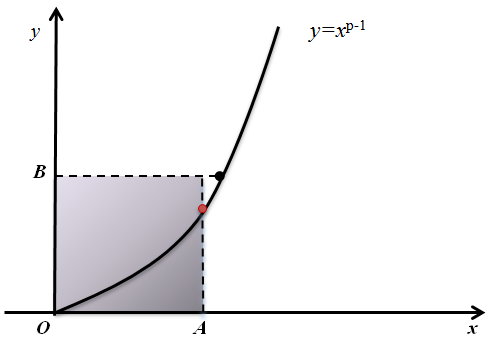
\includegraphics[width=0.65\textwidth]{image/holder.png}
\caption{~利用面积求不等式} \label{fig20}
\end{figure}

可知图~\ref{fig20}~中阴影区域面积恰为~$AB$, 且
\[
AB\leqslant \int_{0}^{A}x^{p-1}\mathrm{d} x+\int_{0}^{B}x^{q-1}\mathrm{d} x
\]
经计算得
\[
AB\leqslant \frac{A^{p}}{p}+\frac{B^{q}}{q}
\]

若~$f$~或~$g$~有一个为零函数, 则不等式~\eqref{equa2}~显然成立. 不妨设~$f$~和~$g$~都不是零函数, 从而
\[
\int_{a}^{b}|f(x)|^{p}\mathrm{d}\mu>0,\quad \int_{a}^{b}|g(x)|^{q}\mathrm{d}\mu>0
\]
由不等式~\eqref{equa3}, 可知
\[ \frac{|f(x)g(x)|}{\Big(\int_{a}^{b}|f(x)|^{p}\mathrm{d}\mu\Big)^{1/p}
\Big(\int_{a}^{b}|g(x)|^{q}\mathrm{d}\mu\Big)^{1/q}}
\leqslant \frac{1}{p}\frac{|f(x)|^{p}}{\int_{a}^{b}|f(x)|^{p}\mathrm{d}\mu}+\frac{1}{q}
\frac{|g(x)|^{q}}{\int_{a}^{b}|g(x)|^{q}\mathrm{d}\mu}
\]
将上式两端取积分后便可得所求不等式~\eqref{equa2}.
\end{proof}

\begin{Theorem}(\textbf{闵可夫斯基不等式}\index{闵可夫斯基不等式})
设~$p\geqslant 1$, $f,\, g\in L^p[a,\,b]$, 则
\begin{equation}\label{equa4}
\Big(\int_{a}^{b}|f(x)+g(x)|^{p}\mathrm{d}\mu\Big)^{\frac{1}{p}}\leqslant \Big(\int_{a}^{b}|f(x)|^{p}\mathrm{d}\mu\Big)^{\frac{1}{p}}+\Big(\int_{a}^{b}|g(x)|^{p}\mathrm{d}\mu\Big)^{\frac{1}{p}}
\end{equation}
\end{Theorem}

\begin{proof}
当~$p=1$~时, 定理显然成立. 设~$p>1$, $q$~为~$p$~的共轭数.

由定理~\ref{thm-2}, $(f(x)+g(x))\in L^p[a,\,b]$, 故~$|f(x)+g(x)|^{\frac{p}{q}}\in L_{q}[a,\,b]$.
将赫德尔不等式中~$g(x)$~换成~$|f(x)+g(x)|^{\frac{p}{q}}$, 可得
\[ \int_{a}^{b}|f(x)|\cdot|f(x)+g(x)|^{\frac{p}{q}}\mathrm{d}\mu
\leqslant \Big(\int_{a}^{b}|f(x)|^{p}\mathrm{d}\mu\Big)^{\frac{1}{p}}\Big(\int_{a}^{b}|f(x)+g(x)|^{p}\mathrm{d}\mu\Big)^{\frac{1}{q}}
\]
同理可知
\[
\int_{a}^{b}|g(x)|\cdot|f(x)+g(x)|^{\frac{p}{q}}\mathrm{d}\mu
\leqslant \Big(\int_{a}^{b}|g(x)|^{p}\mathrm{d}\mu\Big)^{\frac{1}{p}}\Big(\int_{a}^{b}|f(x)+g(x)|^{p}\mathrm{d}\mu\Big)^{\frac{1}{q}}
\]
又
\begin{eqnarray*}
|f(x)+g(x)|^{p}&=&|f(x)+g(x)||f(x)+g(x)|^{\frac{p}{q}}\\
&\leqslant& |f(x)|\cdot|f(x)+g(x)|^{\frac{p}{q}}+|g(x)|\cdot|f(x)+g(x)|^{\frac{p}{q}}
\end{eqnarray*}
因此
\begin{eqnarray*}\label{equa5}
\int_{a}^{b}|f(x)+g(x)|^{p}\mathrm{d}\mu &\leqslant& \Big(\int_{a}^{b}|f(x)|^{p}\mathrm{d}\mu\Big)^{\frac{1}{p}}\Big(\int_{a}^{b}|f(x)+g(x)|^{p}\mathrm{d}\mu\Big)^{\frac{1}{q}}\\
&& + \Big(\int_{a}^{b}|g(x)|^{p}\mathrm{d}\mu\Big)^{\frac{1}{p}}\Big(\int_{a}^{b}|f(x)+g(x)|^{p}\mathrm{d}\mu\Big)^{\frac{1}{q}}
\end{eqnarray*}

当~$\int_{a}^{b}|f(x)+g(x)|^{p}\mathrm{d}\mu\neq 0$~时, 在上述不等式两端都除以
~$\left(\int_{a}^{b}|g(x)|^{p}\mathrm{d}\mu\right)^{\frac{1}{p}}$, 即可得所求不等式~\eqref{equa4}; 当~$\int_{a}^{b}|f(x)+g(x)|^{p}\mathrm{d}\mu=0$~时, 不等式~\eqref{equa4}~自然成立. 定理证毕.
\end{proof}


\subsection*{二、$L^p$~空间的完备性与可分性}

\medskip

\qquad 设~$f(x)\in L^p[a,\,b]$, 定义
\[
\|f\|=\Big(\int_{a}^{b}f^{p}(x)\mathrm{d}\mu \Big)^{\frac{1}{p}}
\]
易知~$\|f\|$~满足范数定义中的性质~(i), (ii), 由闵可夫斯基不等式可知: $\|f\|$~亦满足范数定义中的性质~(iii). 因此, $\|f\|$~确为一范数.

\begin{Remark}
设~$f(x)$~为~$[a,\,b]$~上的可测函数, 若存在零测集~$E_0 \subset [a,\,b]$, 使得~$f(x)$~在~$[a,\,b]-E_0$~上有界．则称~$f(x)$~在~$[a,\,b]$~上本性有界\index{本性有界}. 记
\[
\mathop{\mathrm{ess}\sup}_{x \in [a,b]} f(x) =\inf_{E \subset [a,b] \atop m(E)=0} \Big\{ \sup_{t \in [a,b]-E} | f(x)| \Big\}
\]
称为~$f(x)$~在~$[a,\,b]$~上的本性上确界\index{本性上确界}.

$[a,\,b]$~上本性有界可测函数的全体, 记为~$L^\infty[a,\,b]$\index{$L^\infty$~空间}. 可以证明
\[
\lim_{p \to \infty} \|f\|_p = \|f\|_\infty
\]
事实上, 记~$M = \|f\|_\infty$, 则对任一满足~$M' < M$~的~$M'$, 点集
\[
A = \big\{ x \in [a,\,b]:\: |f(x)| > M'\big\}
\]
有正测度. 由不等式
\[
\|f\|_p = \Big( \int_a^b \big| f(x)\big|^p \mathrm{d} \mu \Big)^\frac{1}{p} \geqslant M' \big( m(A) \big)^\frac{1}{p}
\]
可知
\[
\liminf_{p \to \infty} \|f\|_p \geqslant M'
\]
令~$M' \to M$, 得
\[
\liminf_{p \to \infty} \|f\|_p \geqslant M
\]
另一方面, 我们总有
\[
\|f\|_p \leqslant \Big( \int_a^b M^p \mathrm{d} \mu \Big)^\frac{1}{p} = M \cdot (b-a)^\frac{1}{p}
\]
从而又得
\[
\liminf_{p \to \infty} \|f\|_p \geqslant M
\]
\end{Remark}

下面来看~$L^p[a,\,b]$~的完备性.

\begin{Definition}
设~$(X,\,\|\cdot\|)$~为赋范线性空间, 若对~$X$~中的任意柯西列~$\{x_n\}$, 都存在~$x \in X$, 使得~$x_n \xrightarrow {\|\cdot\|} x$. 则称~$X$~是完备\index{完备}的. 完备的赋范线性空间称为巴拿赫空间\index{巴拿赫空间}.
\end{Definition}

\begin{Theorem}
$L^p[a,\,b]$~空间是完备的, 即对任意柯西列~$\{f_n\} \subset L^p[a,\,b]$, 都存在~$f \in L^p[a,\,b]$~使得~$f_n \xrightarrow {\|\cdot\|} f$.
\end{Theorem}

\begin{proof}
设~$\{f_n\}\subset L^p[a,\,b]$~为柯西列, 则有
\[
\|f_{n}-f_{m}\|\rightarrow 0,\quad n,\,m\rightarrow \infty
\]
即对任意的~$k \in \N$, 存在正整数~$n_{k}$, 当~$n,\,m \geqslant n_{k}$~时, 有
\[
\|f_{n}-f_{m}\|\leqslant \frac{1}{2^{k}}
\]
不妨取~$n_{1}<n_{2}<\cdots$, 从而可得
\[
\sum_{k=1}^{\infty}\|f_{n_{k+1}}-f_{n_{k}}\|\leqslant \sum_{k=1}^{\infty}\frac{1}{2^{k}}=1
\]
令
\[
g_{m}(x)=|f_{n_{1}}(x)|+\sum_{k=1}^{m}|f_{n_{k+1}}(x)-f_{n_{k}}(x)|,\quad m=1,\,2,\,\cdots
\]
则~$g_{m}(x)\in L^p[a,\,b]$. 由范数的性质~(iii)~可知
\[
\|g_{m}\|\leqslant \|f_{n_{1}}\|+\sum_{k=1}^{m}\|f_{n_{k+1}}-f_{n_{k}}\|\leqslant \|f_{n_{1}}\|+1,\quad m=1,\,2,\,\cdots
\]

又~$g_{m}(x)\geqslant 0$~均是可测的, 由法都引理知
\begin{eqnarray*}
\int_{a}^{b}\liminf_{m \to \infty}g_{m}^{p}(x)\mathrm{d}\mu &\leqslant& \liminf_{m \to \infty}\int_{a}^{b}g_{m}^{p}(x)\mathrm{d}\mu \\
&=&\liminf_{m \to \infty}\|g_{m}\|^{p}\leqslant \big(\|f_{n_{1}}\|+1\big)^{p}
\end{eqnarray*}

由于~$\{g_{m}(x)\}$~是单调递增的函数列, 故~$\lim\limits_{m \to \infty}g_{m}(x)$~总存在(有限或者~$+\infty$). 从而
\[
\int_{a}^{b}\lim\limits_{m \to \infty}g_{m}^{p}(x)\mathrm{d}\mu\leqslant \big(\|f_{n_{1}}\|+1 \big)^{p}
\]
由此可知~$\lim\limits_{m \to \infty}g_{m}(x)$~是几乎处处有限的, 即
\[
|f_{n_{1}}(x)|+\sum_{k=1}^{\infty}|f_{n_{k+1}}(x)-f_{n_{k}}(x)|
\]
是几乎处处收敛的. 故函数列
\[
f_{n_{m+1}}(x)=f_{n_{1}}(x)+\sum_{k=1}^{m}(f_{n_{k+1}}(x)-f_{n_{k}}(x)),\quad m=1,\,2,\,\cdots
\]
也是几乎处处收敛的, 故存在几乎处处有限的可测函数~$f(x)$~使得
\[
\lim\limits_{m \to \infty}f_{n_{m}}(x)=f(x),\quad \mbox{~a.e.~} x\in \left[a,\,b\right]
\]
又
\begin{eqnarray*}
|f(x)|&\leqslant & |f_{n_{1}}(x)|+\sum_{k=1}^{\infty}|f_{n_{k+1}}(x)-f_{n_{k}}(x)|\\
&=& \lim\limits_{m \to \infty}g_{m}(x)
\end{eqnarray*}
可知~$f(x)\in L^p[a,\,b]$. 并且
\[
\|f-f_{n_{m}}\|\leqslant \sum_{k=m}^{\infty}\|f_{n_{k+1}}-f_{n_{k}}\| \longrightarrow 0,\quad m\rightarrow \infty
\]
由于
\[
\|f-f_{n}\|\leqslant \|f-f_{n_{m}}\|+\|f_{n}-f_{n_{m}}\|
\]
当~$n\rightarrow \infty$~时, 有
\[
\|f-f_{n}\|\rightarrow 0
\]
定理证毕.
\end{proof}
%%%%%%%%%%%%%%%%%%%%%%可分性%%%%%%%%%%%%%%%%%%%%%%%%%%%%%%%%%%%%%%%%%%%%%%%%%%%%%%%%%%%%%%%%%%%%%%%%

为得到空间~$L^p[a,\,b], p\geqslant 1$~的可分性, 先来介绍下面的一个著名定理:

\smallskip

定义在~$[a,\,b]$~上的所有连续函数的全体记为~$C[a,\,b]$, 设~$f(x)\in C[a,\,b]$, 定义
\[
\|f\|=\sup_{a\leqslant x\leqslant b}|f(x)|
\]
容易验证~$\|f\|$~满足范数定义的三条性质, 确为一范数.

\begin{Theorem}(\textbf{维尔斯特拉斯定理}\index{维尔斯特拉斯定理})
设~$f(x)$~为定义在~$[0,\,1]$~上的连续函数, 并有多项式
\[
B_{n}(x)=\sum_{k=0}^{n}\mathrm{C}_{n}^{k}f(\frac{k}{n})x^{k}(1-x)^{n-k},\quad n=1,\,2,\,\cdots
\]
则
\[
\|B_{n}-f\|=\sup_{0\leqslant  x\leqslant 1}|B_{n}(x)-f(x)| \longrightarrow 0
\]
\end{Theorem}

\begin{proof}
设
\[
b_{n,k}(x)=\mathrm{C}_{n}^{k}x^{k}(1-x)^{n-k},\quad k=1,\,2,\,\cdots, \,n
\]
对~$\forall x\in (0,\,1)$, 有
\[
\sum_{k=0}^{n}b_{n,k}(x)=1
\]
\begin{eqnarray*}
\sum_{k=0}^{n}k b_{n,k}(x)&=& nx\sum_{k=0}^{n}\frac{k}{n}\mathrm{C}_{n}^{k}x^{k-1}(1-x)^{n-k}\\
&=& nx\sum_{k=0}^{n-1}b_{n-1,k}(x)\\
&=& n x
\end{eqnarray*}
\[
\sum_{k=0}^{n}k(k-1) b_{n,k}(x)=n(n-1)x^{2}\sum_{k=0}^{n-2}b_{n-2,k}(x)=n(n-1)x^{2}
\]
因此
\begin{eqnarray*}
\sum_{k=0}^{n}(k-n x)^{2} b_{n,k}(x)&=& n^{2}x^{2}-(2nx-1)nx+n(n-1)x^{2}\\
&=& n x(1-x)
\end{eqnarray*}

由闭区间上连续函数的有界性和一致连续性可知, 存在~$M>0$~使得~$|f(x)|\leqslant M$, 且对任意的~$\varepsilon>0$, 存在~$\delta>0$, 对任意的~$x_{1},\, x_{2}\in [0,\,1]$,
当~$|x_{1}-x_{2}|<\delta$~时, 有
\[
|f(x_{1})-f(x_{2})|<\frac{\varepsilon}{2}
\]
取~$N=\big[M/(\delta^2\varepsilon)+1\big]$, 则
\begin{eqnarray*}
&&\big|B_{n}(x)-f(x)\big|= \Big|\sum_{k=0}^{n}\Big(f(\frac{k}{n})-f(x)\Big) b_{n,k}(x)\Big| \\
&=& \bigg|\sum_{\{k: |\frac{k}{n}-x|\leqslant \delta\}}\Big(f(\frac{k}{n})-f(x)\Big) b_{n,k}(x)+\sum_{\{k: |\frac{k}{n}-x|> \delta\}}\Big(f(\frac{k}{n})-f(x)\Big) b_{n,k}(x)\bigg|\\
&\leqslant& \frac{\varepsilon}{2}\cdot\sum_{k=0}^{n} b_{n,k}(x)+2M\sum_{\{k: |\frac{k}{n}-x|> \delta\}} b_{n,k}(x)\\
&\leqslant& \frac{\varepsilon}{2}+2M\sum_{k=0}^{n}\Big(\frac{k-n x}{n\delta}\Big)^{2}b_{n,k}(x)\\
&=& \frac{\varepsilon}{2}+\frac{2M}{n^{2}\delta^{2}}n x(1-x)\\
&\leqslant& \frac{\varepsilon}{2}+\frac{2M}{n\delta^{2}}\cdot\frac{1}{4} \\
&<&\varepsilon
\end{eqnarray*}
定理证毕.
\end{proof}

\begin{Definition}
设~$(X,\,\|\cdot\|)$~为赋范线性空间, 若~$X$~存在可数的稠密子集, 则称~$X$~是可分\index{可分}的.
\end{Definition}

若~$X$~可分, 则存在一列~$\{x_n\} \subset X$, 使得~$X$~中的每个元~$x$~可以用~$\{x_n\}$~中的元任意逼近, 即存在~$\{x_{n_k}\} \subset \{x_n\}$, 使得~$x_{n_k} \xrightarrow {\|\cdot\|} x$.

\begin{Theorem}
空间~$L^p[a,\,b], p\geqslant 1$~是可分的.
\end{Theorem}

\begin{proof}
对任意的~$f(x)\in L^p[a,\,b]$~及~$\varepsilon>0$, 可知存在有界可测函数列
~$\{f_{N}(x)\}\subset L^p[a,\,b]$~依范数收敛于~$f(x)$. 事实上, 由积分的绝对连续性, 对上述的~$\varepsilon>0$,
存在~$\delta>0$, 当~$m(E)<\delta$~时, 有
\[
\int_{a}^{b}|f(x)|^{p}\mathrm{d}\mu<(\frac{\varepsilon}{3})^{p}
\]
又因~$f(x)$~是几乎处处有限的可测函数, 故对上述的~$\delta>0$, 存在自然数~$N$, 使得
\[
m\big(\{x\in [a,\,b]:\: |f(x)|>N \}\big)<\delta
\]
令
\[
f_{N}(x)= \left\{\!\!
\begin{array}{cl}
f(x), & \quad |f(x)|<N \\[0.2cm]
0, & \quad |f(x)|\geqslant N
\end{array}
\right.
\]
显然, $f_{N}(x)\in L^p[a,\,b]$~是有界的, 且
\begin{eqnarray*}
\|f-f_{N}\|&=&\Big(\int_{a}^{b}|f(x)-f_{N}(x)|^{p}\mathrm{d}\mu\Big)^{\frac{1}{p}}\\
&=&\Big(\int_{\{x\in \left[a,\,b\right]:\: |f(x)|>N \}}|f(x)-f_{N}(x)|^{p}\mathrm{d}\mu\Big)^{\frac{1}{p}}<\frac{\varepsilon}{3}
\end{eqnarray*}
由卢津定理, 可知对每个有界可测函数~$f_{N}(x)$, 存在连续函数~$g_{N}(x)$~使得
\[
|g_{N}(x)|\leqslant N
\]
\[
m\big(\{x\in [a,\,b]:\: f_{N}(x)\neq g_{N}(x)\}\big)<\Big(\frac{\varepsilon}{6N}\Big)^{p}
\]
记~$E_0 = \{x\in [a,\,b]:\: f_{N}(x)\neq g_{N}(x)\}$, 从而
\begin{eqnarray*}
\|f_{N}-g_{N}\| &=& \Big(\int_{a}^{b}|f_{N}(x)-g_{N}(x)|^{p}\mathrm{d}\mu\Big)^{\frac{1}{p}}\\
&=&\left(\int_{E_0}|f_{N}(x)-g_{N}(x)|^{p}\mathrm{d}\mu\right)^{\frac{1}{p}}\\
&\leqslant& \Big(\int_{E_0}|f_{N}(x)|^{p}\mathrm{d}\mu\Big)^{\frac{1}{p}}
+ \Big(\int_{E_0}|g_{N}(x)|^{p}\mathrm{d}\mu\Big)^{\frac{1}{p}}\\
&\leqslant& \big[N^{p}\cdot m\big(E_0\big)\big]^{\frac{1}{p}}
+\big[N^{p}\cdot m\big(E_0\big)\big]^{\frac{1}{p}} \\
&<&\frac{\varepsilon}{3}
\end{eqnarray*}
再根据维尔斯特拉斯定理, 连续函数~$g_{N}(x)$~可由有理系数多项式一致逼近, 即存在有理系数多项式~$P_{N}(x)$~使得
\[
\max_{x\in [a,\,b]}|g_{N}(x)-P_{N}(x)|<\frac{\varepsilon}{3(b-a)^{1/p}}
\]
从而
\[
\|g_{N}-P_{N}\|=\Big(\int_{a}^{b}|g_{N}(x)-P_{N}(x)|^{p}\mathrm{d}\mu\Big)^{\frac{1}{p}}\leqslant \frac{\varepsilon}{3}
\]
则
\begin{eqnarray*}
\|f-P_{n}\|&\leqslant& \|f-f_{N}\|+\|f_{N}-g_{N}\|+\|g_{N}-P_{N}\|\\
&<&\frac{\varepsilon}{3}+\frac{\varepsilon}{3}+\frac{\varepsilon}{3}=\varepsilon
\end{eqnarray*}
因此, $[a,\,b]$~上的有理系数多项式在~$L^p[a,\,b]$~上是稠密的, 而所有有理系数多项式构成的集合是可数的, 故定理成立.
\end{proof}

\newpage

\vspace*{-0.6cm}

\section*{第六章习题}

%\addcontentsline{toc}{section}{~~~~~第六章习题}

\begin{enumerate}

\item 设~$f_{n}(x), f(x)\in L^2[a,\,b]$, $f_{n}$~依测度收敛于~$f$, 若存在~$M>0$~使得~$\|f_{n}\|\leqslant M$, 试证明~$f_{n}$~弱收敛于~$f$.

\item 设~$f_{n}(x), f(x)\in L^2[a,\,b]$, $f_{n}$~弱收敛于~$f$, 则存在~$M>0$~使得~$\|f_{n}\|\leqslant M$.

\item 举例说明~$L^2[a,\,b]$~中的弱收敛函数列未必是依测度收敛的.

\item 若对任意的~$f(x)\in L^2[a,\,b]$, 都有
\[
\int_{a}^{b}f(x)g(x)\mathrm{d}\mu<\infty
\]
则~$g(x) \in L^2[a,\,b]$.

\item 设~$f_{n}(x), f(x)\in L^2[a,\,b]$, $f_{n}$~弱收敛于~$f$, 且~$\|f_{n}\|\rightarrow \|f\|$, 则~$f_{n}$~依范数收敛于~$f$.

\item 试证明~$L^2[a,\,b]$~中的规范正交系至多是可数的.

\item 设~$\{g_{n}(x)\}$~是定义在~$\left[a,\,b\right]$~上封闭的规范正交系, 则~$\sum\limits_{n=1}^{\infty}g_{n}^{2}(x)=+\infty$~在~$\left[a,\,b\right]$~上几乎处处成立.


\item 设~$\{g_{n}(x)\}\subset L^2[a,\,b]$~是完全的规范正交系, 若~$\{\varphi_{n}(x)\}\subset L^2[a,\,b]$~满足
\[
\sum_{n=1}^{\infty}\int_{a}^{b}[g_{n}(x)-\varphi_{n}(x)]^{2}\mathrm{d}\mu<1
\]
则~$\{\varphi_{n}(x)\}$~也是完全的.

\item 试证明~$L^2[a,\,b]$~中有限的函数系不是完全的.

\item 设~$\{g_{n}(x)\}\subset L^2[a,\,b]$~是一规范正交系, $f(x)\in L^2[a,\,b]$. 对线性组合~$\sum\limits_{k=1}^{n}a_{k}g_{k}(x)$~作范数
\[
\Big\|f-\sum_{k=1}^{n}a_{k}g_{k}\Big\|
\]
则当~$a_{k}=(f,g_{k})$~时, 上述范数取最小值.

\item 试证明~$L^p[a,\,b], p\geqslant 1$~是完全的.

\item 设~$f\in L^p[a,\,b]\cap L^{p'}\left[a,\,b\right]$, $1\leqslant p<r<p'$, 试证明~$f\in L^{r}\left[a,\,b\right]$.

\item 设~$f \in L^p(E)$, $e \subset E$~可测, 证明
\[
\Big( \int_E |f(x)|^p \mathrm{d} \mu \Big)^\frac{1}{p} \leqslant \Big( \int_e |f(x)|^p \mathrm{d} \mu \Big)^\frac{1}{p} + \Big( \int_{E-e} |f(x)|^p \mathrm{d} \mu \Big)^\frac{1}{p}
\]

\item 设~$f \in L^p(-\infty,\,+\infty),\,g\in L^q(-\infty,\,+\infty)$, 其中~$\frac{1}{p}+\frac{1}{q} =1,\,p\geqslant 1$, 试证
    \[
    F(t)=\int_{-\infty}^{+\infty} f(x+t)g(x) \mathrm{d} \mu
    \]
    为~$t$~的连续函数.

\item 设~$f_{n}(x),\, f(x)\in L^p[a,\,b], p\geqslant 1$, 若~$f_{n}\xrightarrow{\mathrm{\|\cdot\|}} f$, 则~$\{f_n\}$~是柯西列.

\item 设~$f_{n}(x),\, f(x)\in L^p[a,\,b], p\geqslant 1$, 若~$f_{n}\xrightarrow{\mathrm{\|\cdot\|}} f$, 则~$\|f_n\|\rightarrow \|f\|$.

\item $L^p[a,\,b], p\geqslant 1$~中的函数列在依范数收敛的意义下, 极限函数是唯一的.

\item 设~$f\in L^p[a,\,b], p\geqslant 1$, 则对任意~$\varepsilon>0$, 存在有界可测函数~$g$~使得
\[
\|f-g\|<\varepsilon
\]

\item 设~$f\in L^p[a,\,b], p\geqslant 1$, 则对任意~$\varepsilon>0$, 存在连续函数~$F$~使得
\[
\|f-F\|<\varepsilon
\]

\end{enumerate}